\documentclass{tufte-book}

\hypersetup{colorlinks}% uncomment this line if you prefer colored hyperlinks (e.g., for onscreen viewing)

%%
% If they're installed, use Bergamo and Chantilly from www.fontsite.com.
% They're clones of Bembo and Gill Sans, respectively.
%\IfFileExists{bergamo.sty}{\usepackage[osf]{bergamo}}{}% Bembo
%\IfFileExists{chantill.sty}{\usepackage{chantill}}{}% Gill Sans

%\usepackage{microtype}

\usepackage[final]{pdfpages}

\usepackage{tikz}
\usetikzlibrary{arrows,calc,decorations.markings,positioning,shadows,shapes,trees}

\tikzset{
  basic/.style  = {draw, text width=2cm, drop shadow, font=\sffamily, rectangle},
  root/.style   = {basic, text width=5cm, rounded corners=2pt, thin, align=center,
                   fill=green!30},
  level 2/.style = {basic, rounded corners=6pt, thin,align=center, fill=green!60,
                   text width=8em},
  level 3/.style = {basic, thin, align=left, fill=pink!60, text width=6.5em}
}

\usepackage{pgffor}

\usepackage{verbatim}

\usepackage{hyperref}


%%
% Just some sample text
\usepackage{lipsum}

%%
% For nicely typeset tabular material
\usepackage{booktabs}

%%
% For graphics / images
\usepackage{graphicx}
\setkeys{Gin}{width=\linewidth,totalheight=\textheight,keepaspectratio}
\graphicspath{{graphics/}}

% The fancyvrb package lets us customize the formatting of verbatim
% environments.  We use a slightly smaller font.
\usepackage{fancyvrb}
\fvset{fontsize=\normalsize}

%%
% Prints argument within hanging parentheses (i.e., parentheses that take
% up no horizontal space).  Useful in tabular environments.
\newcommand{\hangp}[1]{\makebox[0pt][r]{(}#1\makebox[0pt][l]{)}}

%%
% Prints an asterisk that takes up no horizontal space.
% Useful in tabular environments.
\newcommand{\hangstar}{\makebox[0pt][l]{*}}

%%
% Prints a trailing space in a smart way.
\usepackage{xspace}

%%
% Some shortcuts for Tufte's book titles.  The lowercase commands will
% produce the initials of the book title in italics.  The all-caps commands
% will print out the full title of the book in italics.
\newcommand{\vdqi}{\textit{VDQI}\xspace}
\newcommand{\ei}{\textit{EI}\xspace}
\newcommand{\ve}{\textit{VE}\xspace}
\newcommand{\be}{\textit{BE}\xspace}
\newcommand{\VDQI}{\textit{The Visual Display of Quantitative Information}\xspace}
\newcommand{\EI}{\textit{Envisioning Information}\xspace}
\newcommand{\VE}{\textit{Visual Explanations}\xspace}
\newcommand{\BE}{\textit{Beautiful Evidence}\xspace}

\newcommand{\TL}{Tufte-\LaTeX\xspace}

% Prints the month name (e.g., January) and the year (e.g., 2008)
\newcommand{\monthyear}{%
  \ifcase\month\or January\or February\or March\or April\or May\or June\or
  July\or August\or September\or October\or November\or
  December\fi\space\number\year
}


% Prints an epigraph and speaker in sans serif, all-caps type.
\newcommand{\openepigraph}[2]{%
  %\sffamily\fontsize{14}{16}\selectfont
  \begin{fullwidth}
  \sffamily\large
  \begin{doublespace}
  \noindent\allcaps{#1}\\% epigraph
  \noindent\allcaps{#2}% author
  \end{doublespace}
  \end{fullwidth}
}

% Inserts a blank page
\newcommand{\blankpage}{\newpage\hbox{}\thispagestyle{empty}\newpage}

\usepackage{units}

% Typesets the font size, leading, and measure in the form of 10/12x26 pc.
\newcommand{\measure}[3]{#1/#2$\times$\unit[#3]{pc}}

% Macros for typesetting the documentation
\newcommand{\hlred}[1]{\textcolor{Maroon}{#1}}% prints in red
\newcommand{\hangleft}[1]{\makebox[0pt][r]{#1}}
\newcommand{\hairsp}{\hspace{1pt}}% hair space
\newcommand{\hquad}{\hskip0.5em\relax}% half quad space
\newcommand{\TODO}{\textcolor{red}{\bf TODO!}\xspace}
\newcommand{\ie}{\textit{i.\hairsp{}e.}\xspace}
\newcommand{\eg}{\textit{e.\hairsp{}g.}\xspace}
\newcommand{\na}{\quad--}% used in tables for N/A cells
\providecommand{\XeLaTeX}{X\lower.5ex\hbox{\kern-0.15em\reflectbox{E}}\kern-0.1em\LaTeX}
\newcommand{\tXeLaTeX}{\XeLaTeX\index{XeLaTeX@\protect\XeLaTeX}}
% \index{\texttt{\textbackslash xyz}@\hangleft{\texttt{\textbackslash}}\texttt{xyz}}
\newcommand{\tuftebs}{\symbol{'134}}% a backslash in tt type in OT1/T1
\newcommand{\doccmdnoindex}[2][]{\texttt{\tuftebs#2}}% command name -- adds backslash automatically (and doesn't add cmd to the index)
\newcommand{\doccmddef}[2][]{%
  \hlred{\texttt{\tuftebs#2}}\label{cmd:#2}%
  \ifthenelse{\isempty{#1}}%
    {% add the command to the index
      \index{#2 command@\protect\hangleft{\texttt{\tuftebs}}\texttt{#2}}% command name
    }%
    {% add the command and package to the index
      \index{#2 command@\protect\hangleft{\texttt{\tuftebs}}\texttt{#2} (\texttt{#1} package)}% command name
      \index{#1 package@\texttt{#1} package}\index{packages!#1@\texttt{#1}}% package name
    }%
}% command name -- adds backslash automatically
\newcommand{\doccmd}[2][]{%
  \texttt{\tuftebs#2}%
  \ifthenelse{\isempty{#1}}%
    {% add the command to the index
      \index{#2 command@\protect\hangleft{\texttt{\tuftebs}}\texttt{#2}}% command name
    }%
    {% add the command and package to the index
      \index{#2 command@\protect\hangleft{\texttt{\tuftebs}}\texttt{#2} (\texttt{#1} package)}% command name
      \index{#1 package@\texttt{#1} package}\index{packages!#1@\texttt{#1}}% package name
    }%
}% command name -- adds backslash automatically
\newcommand{\docopt}[1]{\ensuremath{\langle}\textrm{\textit{#1}}\ensuremath{\rangle}}% optional command argument
\newcommand{\docarg}[1]{\textrm{\textit{#1}}}% (required) command argument
\newenvironment{docspec}{\begin{quotation}\ttfamily\parskip0pt\parindent0pt\ignorespaces}{\end{quotation}}% command specification environment
\newcommand{\docenv}[1]{\texttt{#1}\index{#1 environment@\texttt{#1} environment}\index{environments!#1@\texttt{#1}}}% environment name
\newcommand{\docenvdef}[1]{\hlred{\texttt{#1}}\label{env:#1}\index{#1 environment@\texttt{#1} environment}\index{environments!#1@\texttt{#1}}}% environment name
\newcommand{\docpkg}[1]{\texttt{#1}\index{#1 package@\texttt{#1} package}\index{packages!#1@\texttt{#1}}}% package name
\newcommand{\doccls}[1]{\texttt{#1}}% document class name
\newcommand{\docclsopt}[1]{\texttt{#1}\index{#1 class option@\texttt{#1} class option}\index{class options!#1@\texttt{#1}}}% document class option name
\newcommand{\docclsoptdef}[1]{\hlred{\texttt{#1}}\label{clsopt:#1}\index{#1 class option@\texttt{#1} class option}\index{class options!#1@\texttt{#1}}}% document class option name defined
\newcommand{\docmsg}[2]{\bigskip\begin{fullwidth}\noindent\ttfamily#1\end{fullwidth}\medskip\par\noindent#2}
\newcommand{\docfilehook}[2]{\texttt{#1}\index{file hooks!#2}\index{#1@\texttt{#1}}}
\newcommand{\doccounter}[1]{\texttt{#1}\index{#1 counter@\texttt{#1} counter}}

%%%
\title{\textbf{Seeker\\\normalsize{Documentation}}}
\author{Jaroslaw Hirniak}
\date{Last updated on: \emph{\today}}
\setcounter{tocdepth}{1}

% Generates the index
\usepackage{makeidx}
\makeindex

\begin{document}

\maketitle

\tableofcontents

%--- Ch1: Project
\chapter{Project}
 
\section{Motivation}
\paragraph{}
The World Wide Web is a very rich source of information and many excellent search engines exist that help to find interesting information in the matters of milliseconds. However, they only provide links to the source of information and if user wants to compare data from many sources or gather it for analysis purpose they are left with a daunting task of collecting all this information by hand.

\paragraph{}
This is repetitive and boring task, something that humans do not enjoy, but computers excel in. It would be of significant help to any researchers that need to compare vast sections of information from multitude of sources to have a tool that would take care of the first part of the analysis, which is collection of relevant data, and let the researcher to concentrate on what is important and hard - the reasoning about the data.

\paragraph{}
The goal of this project is to research feasibility of implementing a system for querying big data sets (e.g. collection of 100 pages report from standardization committee) and presenting only relevant sections of it (e.g. only few paragraphs of interest filtered from across a thousand of related documents stored in the database).  The last step of the project is to implement a proof of concept system that possibly could be developed into fully functional system.

\section{Feasibility and technologies}
\paragraph{}
The first part of the project is going to be to investigate the nature of the problem and if it can be efficiently solved. If it can be solved then suitable technologies will be suggested and used in the proof of concept system.

\section{Proof of concept}
\paragraph{}
The project idea originated from a problem common to the researches in minority languages at the University of Edinburgh, who faced issue of gathering data from variety of sources, for instance from \href{http://www.coe.int/t/dg4/education/minlang/Report/default_en.asp}{European Charter for Regional or Minority Languages} website for comparative analysis and producing various reports based on that data. However, the problem is that data is presented in PDF reports (and is not annotated in anyway), the layout of reports vary (depending on the cycle, country issuing it, and other factors), and average length of a report is over 100 pages. Thus, any researcher interested in using valuable data from reports must face first daunting extraction of interesting information sections from multiple sources.

\section{Data sources}
\paragraph{}
The primary intended source of data are long documents, often being reports, with usual length from 50 to 100 pages, in different formats like DOC(X), ODT, PDF, TXT, etc. and being unannounced beside in the most optimistic case having similar structure across range of documents. For example, for the proof of concept there are 651 PDF documents listed on the page, of which 309 documents are in English (some documents are produced also in French or country producing report official language), of which 300 documents are of actual interest (rest includes charter advertisements or documents that do not present valuable source of information). There are 25 countries producing reports, each adhering to general layout, but with subtle differences coming from the tool used or typesetting conventions, which should be taken into account during parsing PDF into JSON\footnote{Thus, the optimal parser would be context aware (and such parser was implemented for this project).}.

\section{Stakeholders}

Each of the stakeholders is important part of the system without which the system could not be considered successful, all with different needs, and assumptions about the system functionality.

\begin{itemize}
  \item Researchers - people who are using service often for their research and rely on the correctness and up-to-date properties of the system;
  \item Consumers - people who need to access data occasionally and do not have need to register an account in the service, or even do not care if the document published 2 days ago is included in the search;
  \item Administrators - people having rights to add sources, respond to tickets, etc., and responsible for the service maintenance;
  \item Developer - person responsible for the project development and code base maintenance.
\end{itemize}

\section{Project Name}
The project name \emph{Seeker} comes from \href{http://www.scottishpoetrylibrary.org.uk/poetry/poems/seeker-reaper}{``Seeker, Reaper''} poem by \href{http://en.wikipedia.org/wiki/George_Campbell_Hay}{George Campbell Hay}. You can listen to the peom being recited on YouTube \href{https://www.youtube.com/watch?v=gjxPtRZFF24}{here}.

%---

%--- Ch2: Requirements

\chapter{Requirements}

\section{Summer 2014 plan}
The goal for 8 week summer project was set to
\begin{itemize}
  \item carry out research and recommend appropriate solution (architecture, full software stack, and persistence layer);
  \item Implement a proof of concept functionality to prove the possibility of developing efficient solution for the stated problem, this is, ability to query European Committee for Minority Languages and receive combined documents composed of elements specified in the query.
  \item Deploy the proof of concept on the university server for evaluation and presentation.
\end{itemize}

\section{Data format}
The main source of the data are going to be the European Charter for Regional or Minority Languages expert reports\footnote{\url{http://www.coe.int/t/dg4/education/minlang/Report/default_en.asp}}.

The goal of the project is to account for the future grow and to include also documents from Galeic Plans produced by various bodies in Scotland \footnote{http://www.gaidhlig.org.uk/bord/en/our-work/gaelic-language-plans.php}.

The data needs to be assumed to do not have any common format or fields.

\section{Use cases}
During the initial meeting on 26 May 2014 the below use cases were identified.

\begin{figure*}[h] 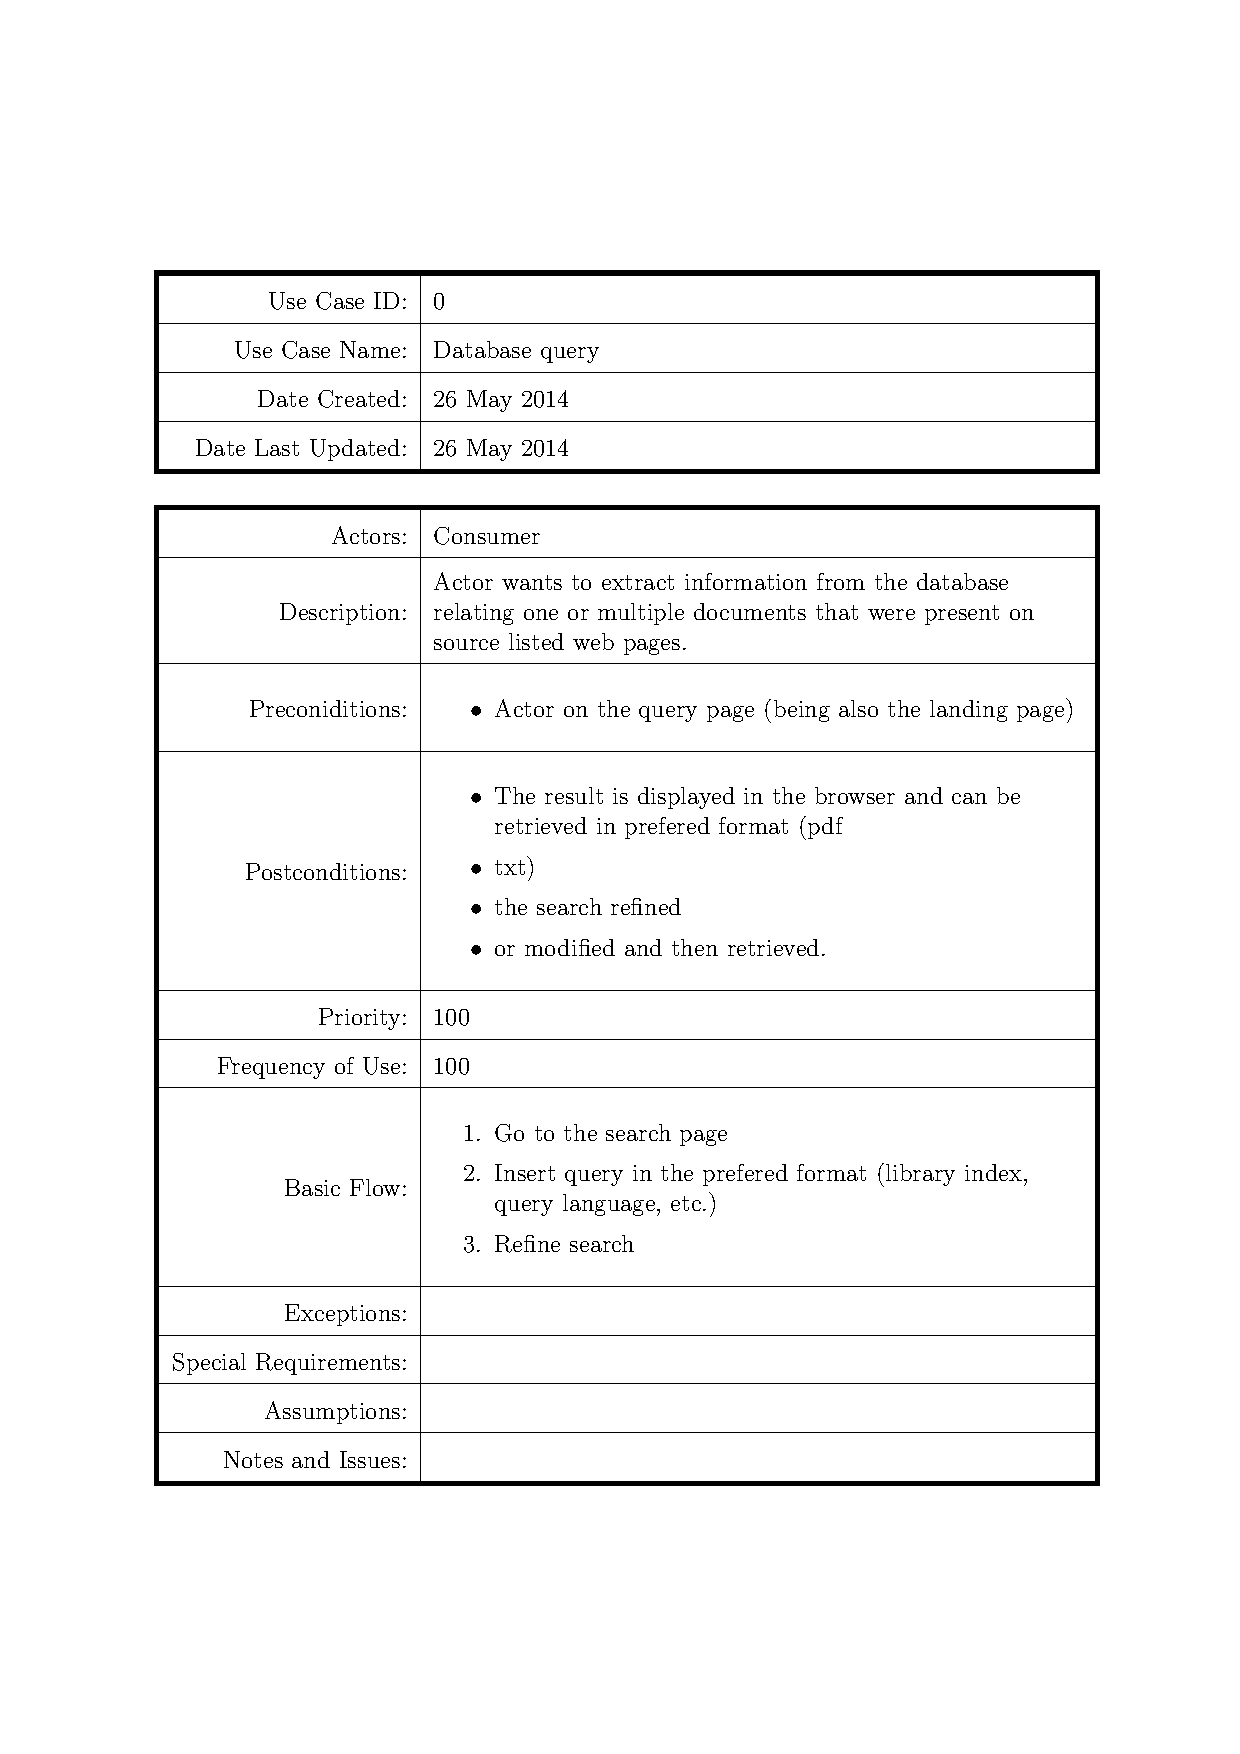
\includegraphics[width=\linewidth]{Requirements/UseCases/000_Query.pdf}\end{figure*}
\begin{figure*}[h] 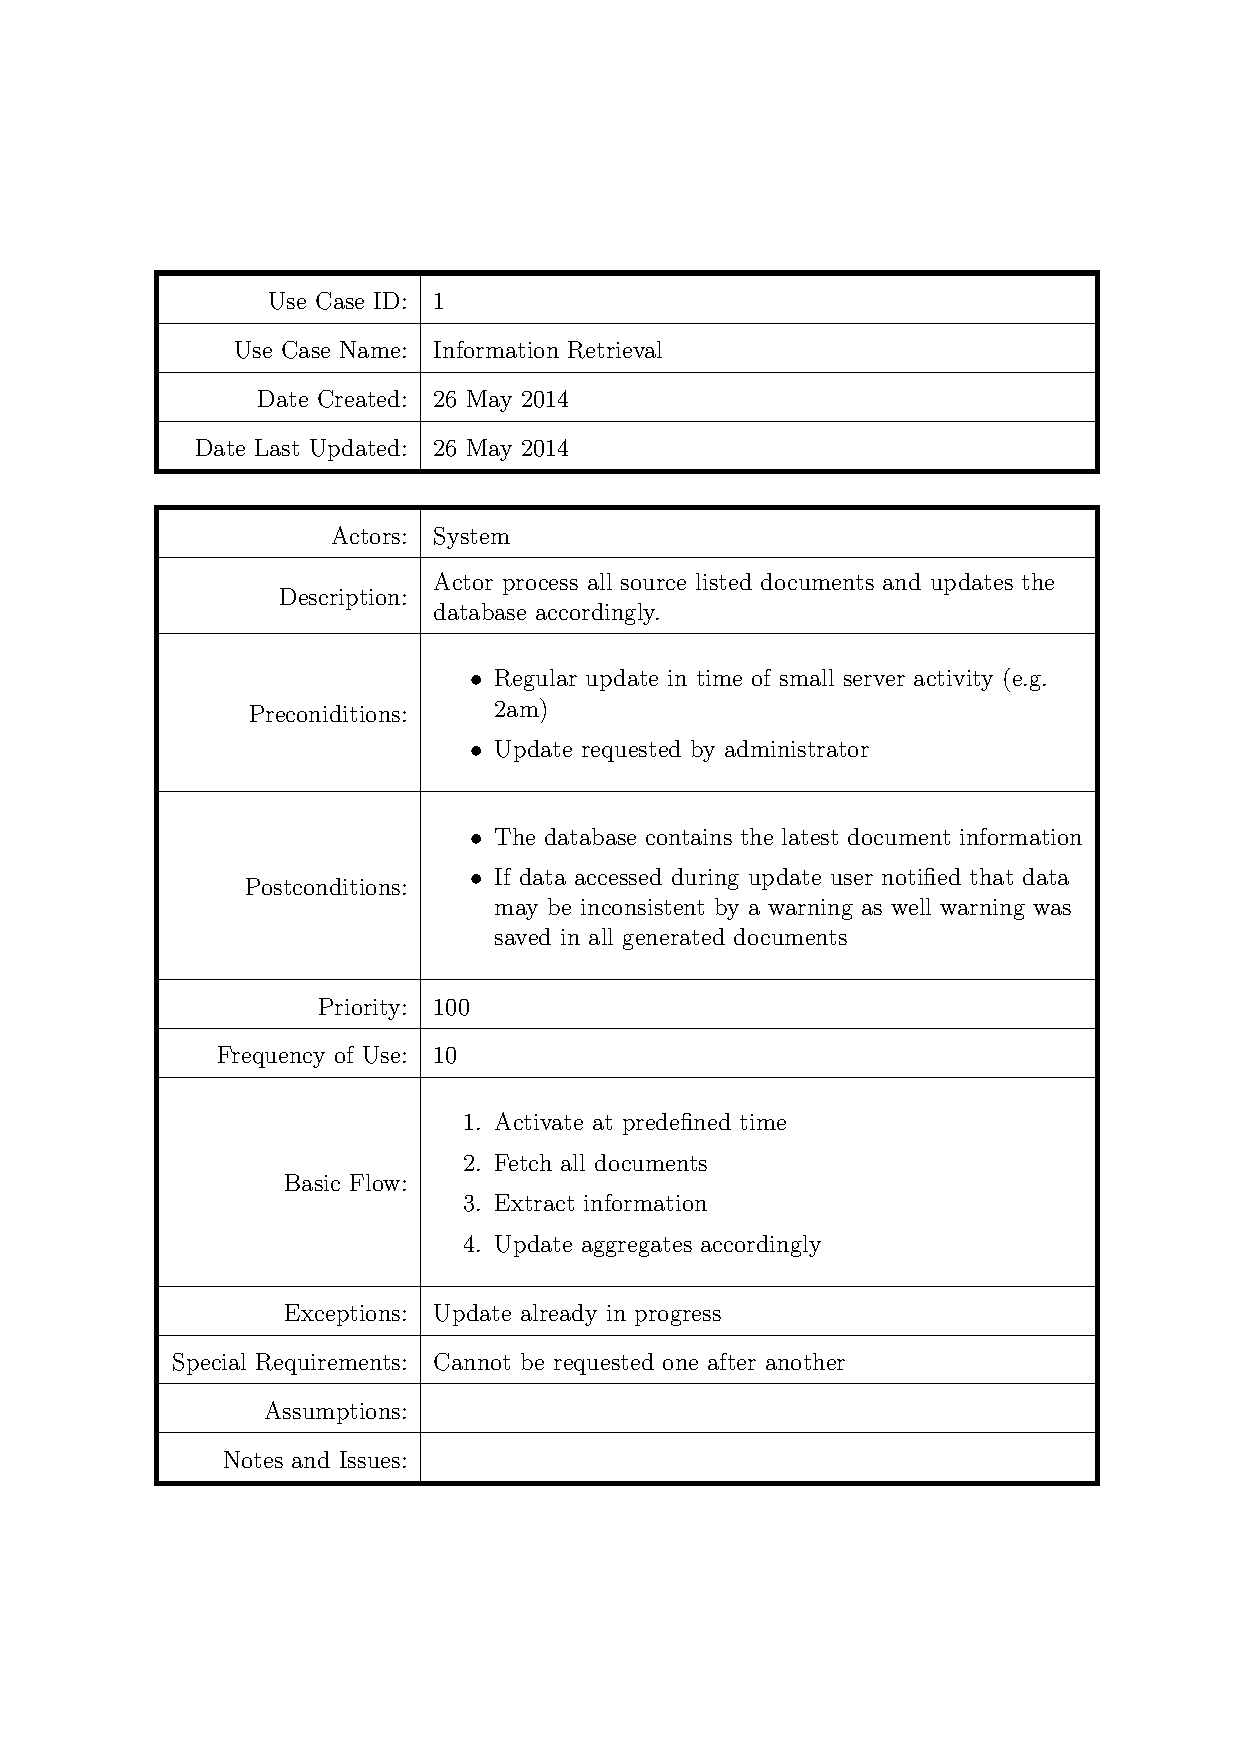
\includegraphics[width=\linewidth]{Requirements/UseCases/001_IR.pdf}\end{figure*}
\begin{figure*}[h] 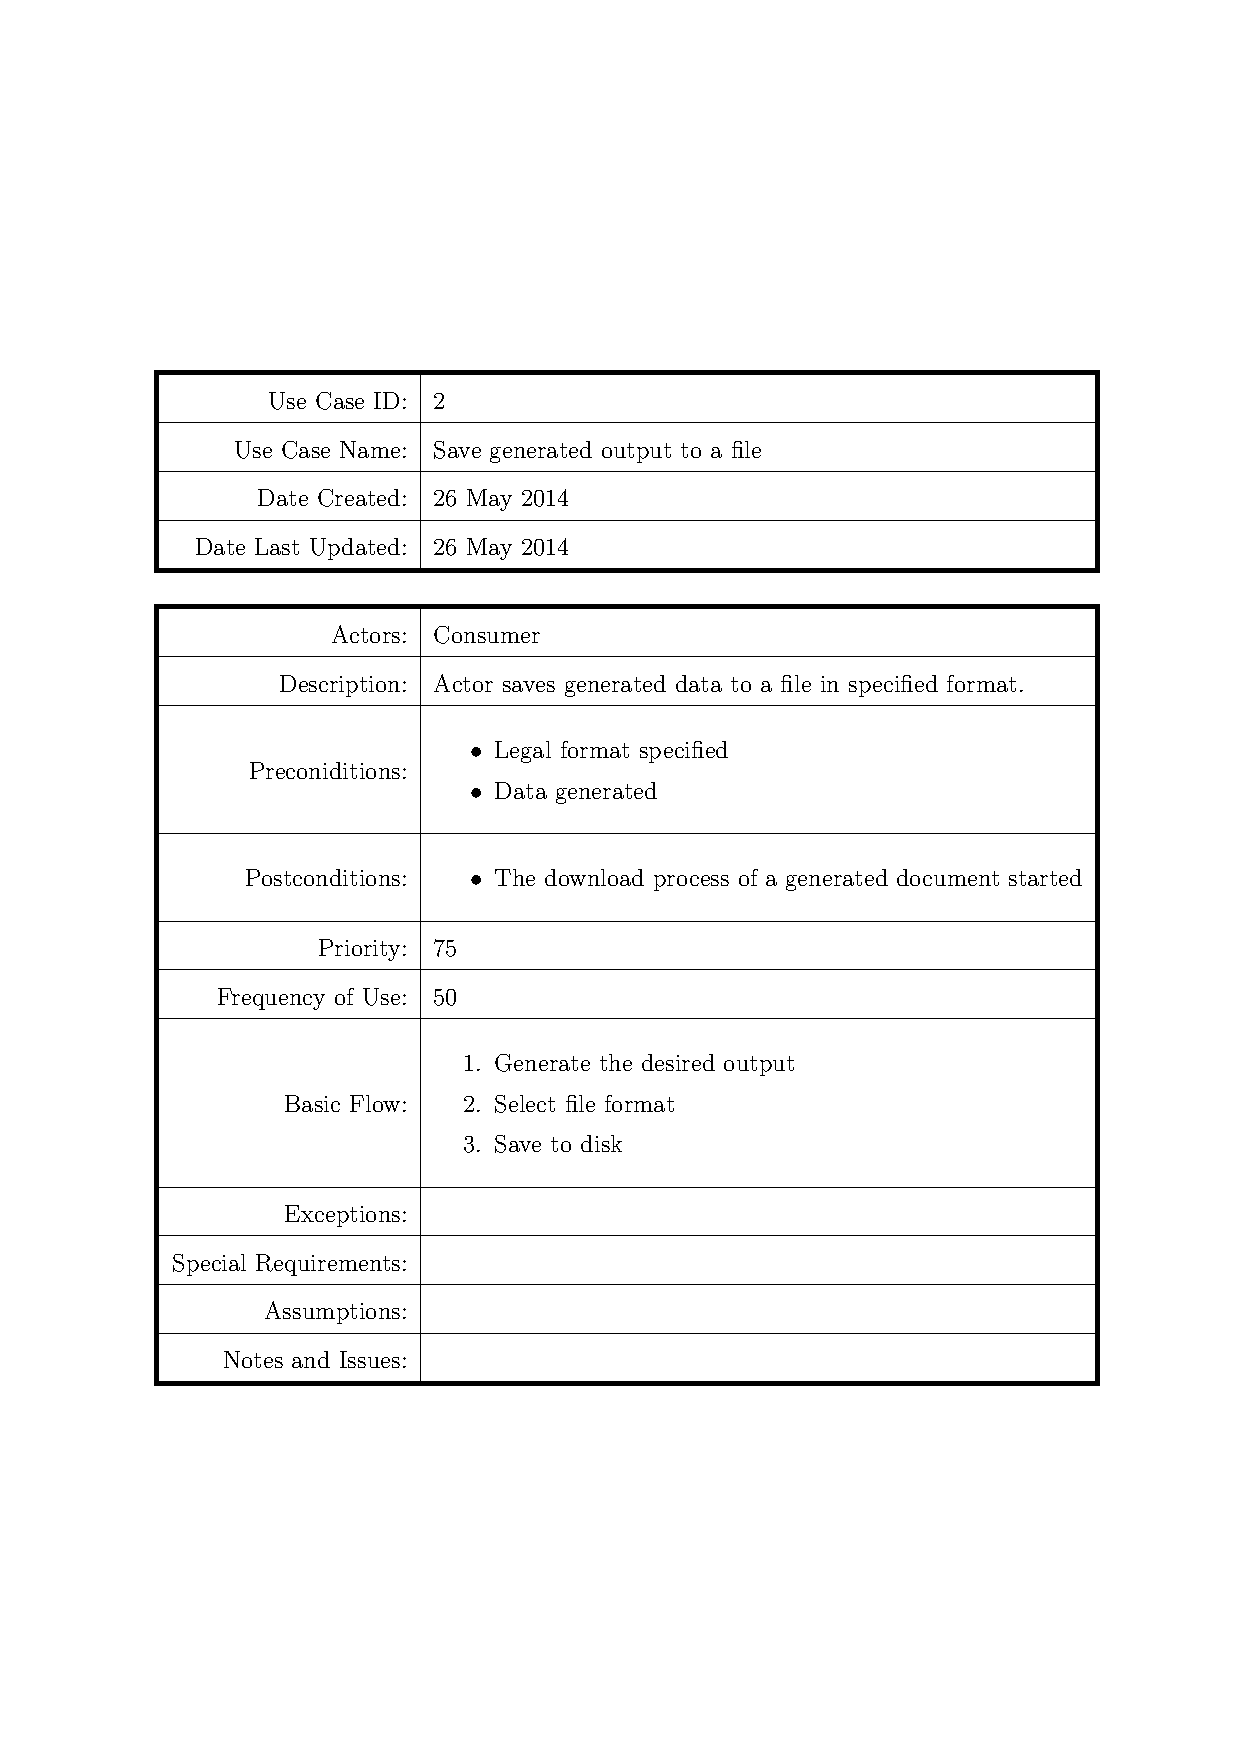
\includegraphics[width=\linewidth]{Requirements/UseCases/002_SaveOutput2File.pdf}\end{figure*}
\begin{figure*}[h] 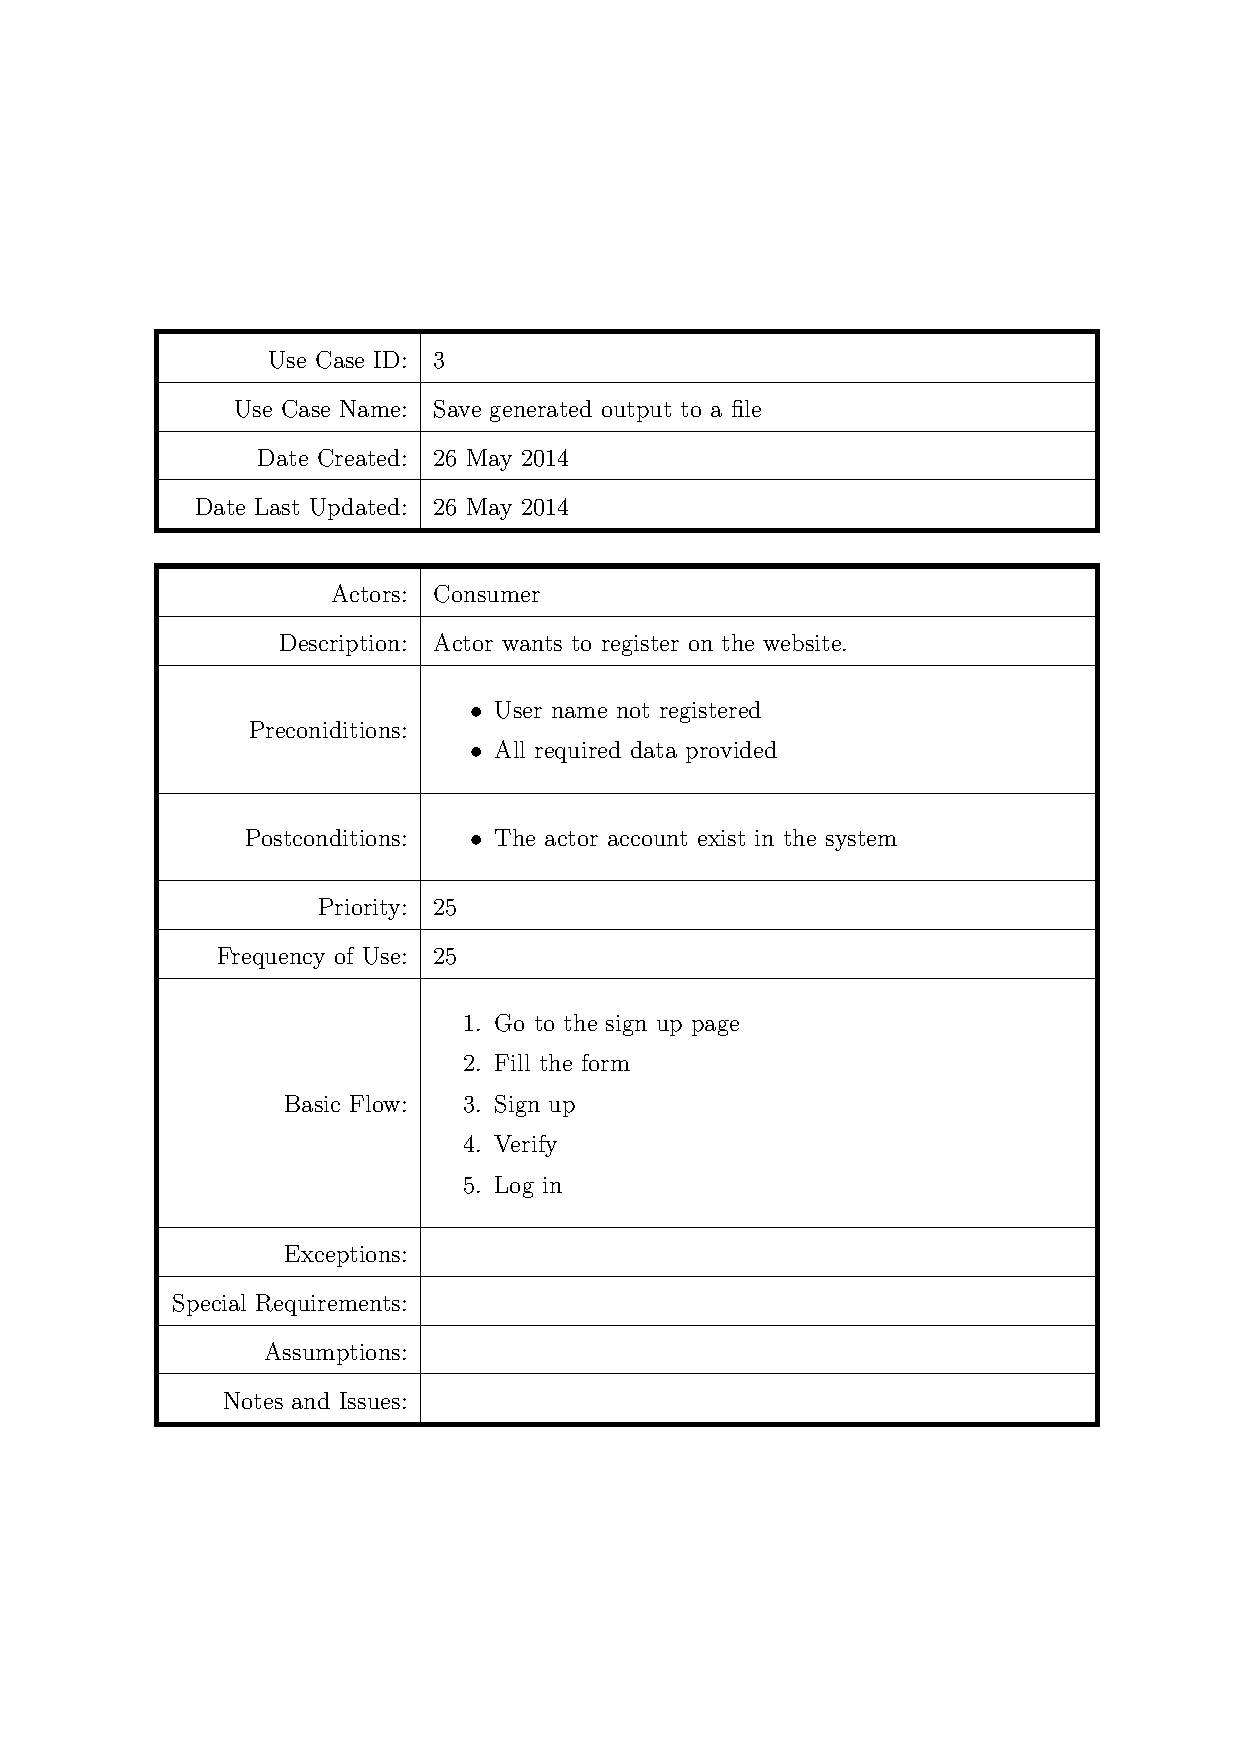
\includegraphics[width=\linewidth]{Requirements/UseCases/003_SignUp.pdf}\end{figure*}
\begin{figure*}[h] 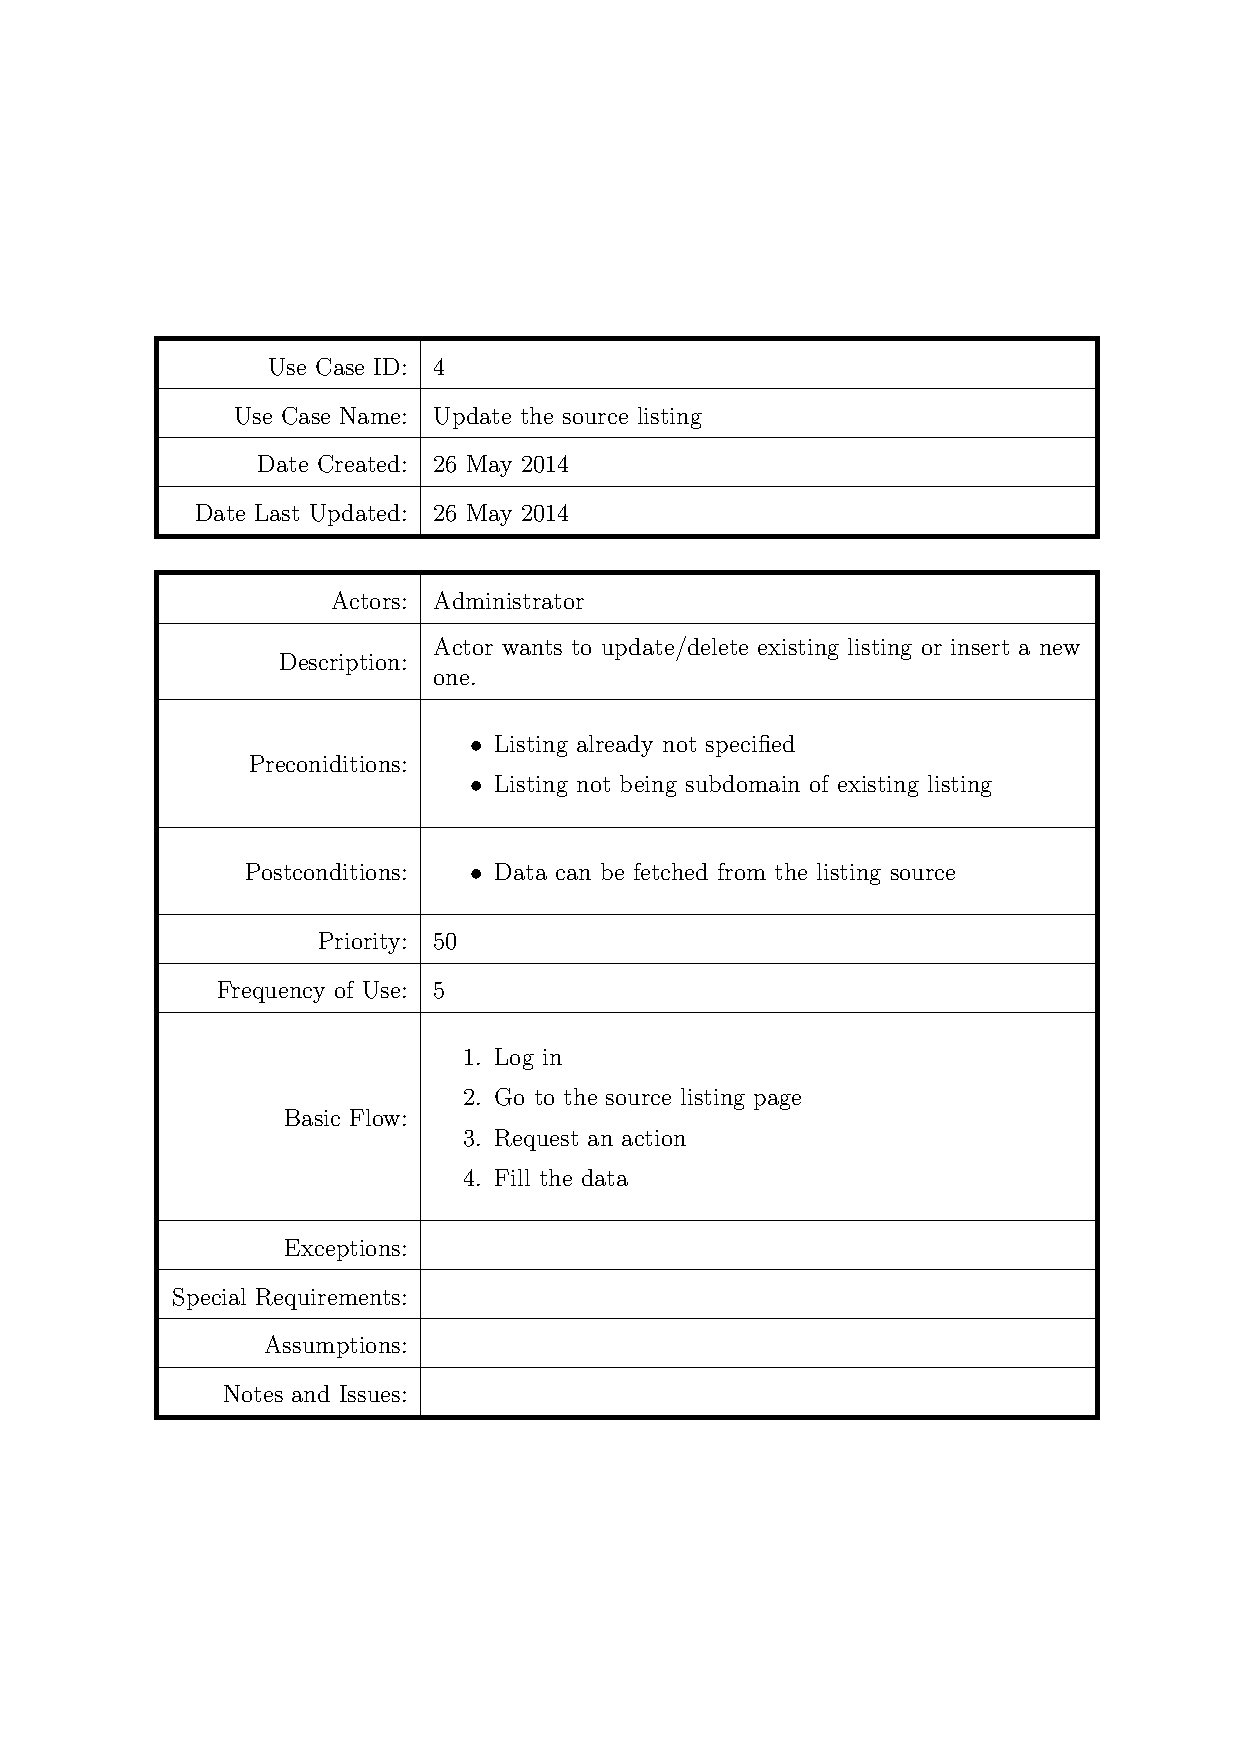
\includegraphics[width=\linewidth]{Requirements/UseCases/004_SourceListingUpdate.pdf}\end{figure*}
\begin{figure*}[h] 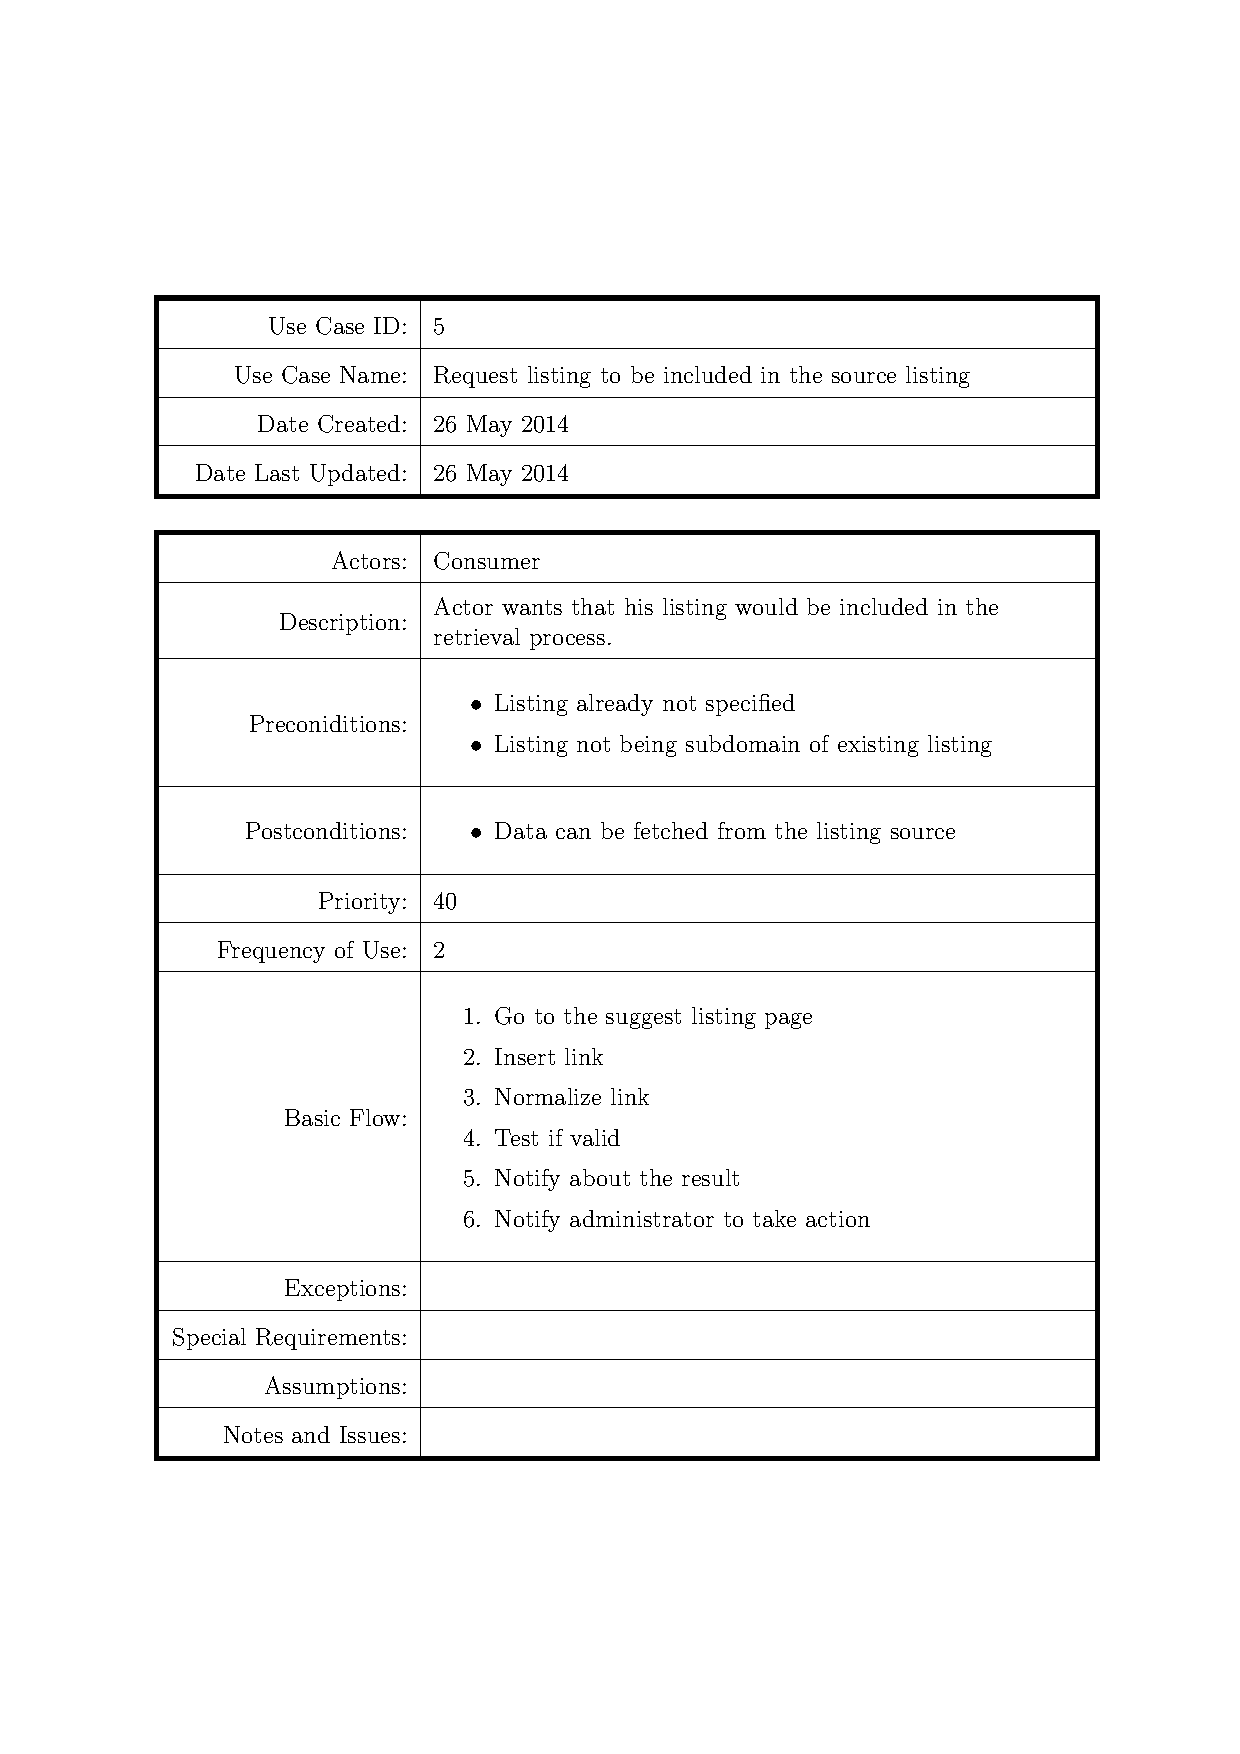
\includegraphics[width=\linewidth]{Requirements/UseCases/005_RequestListingToBeIncluded.pdf}\end{figure*}
\begin{figure*}[h] 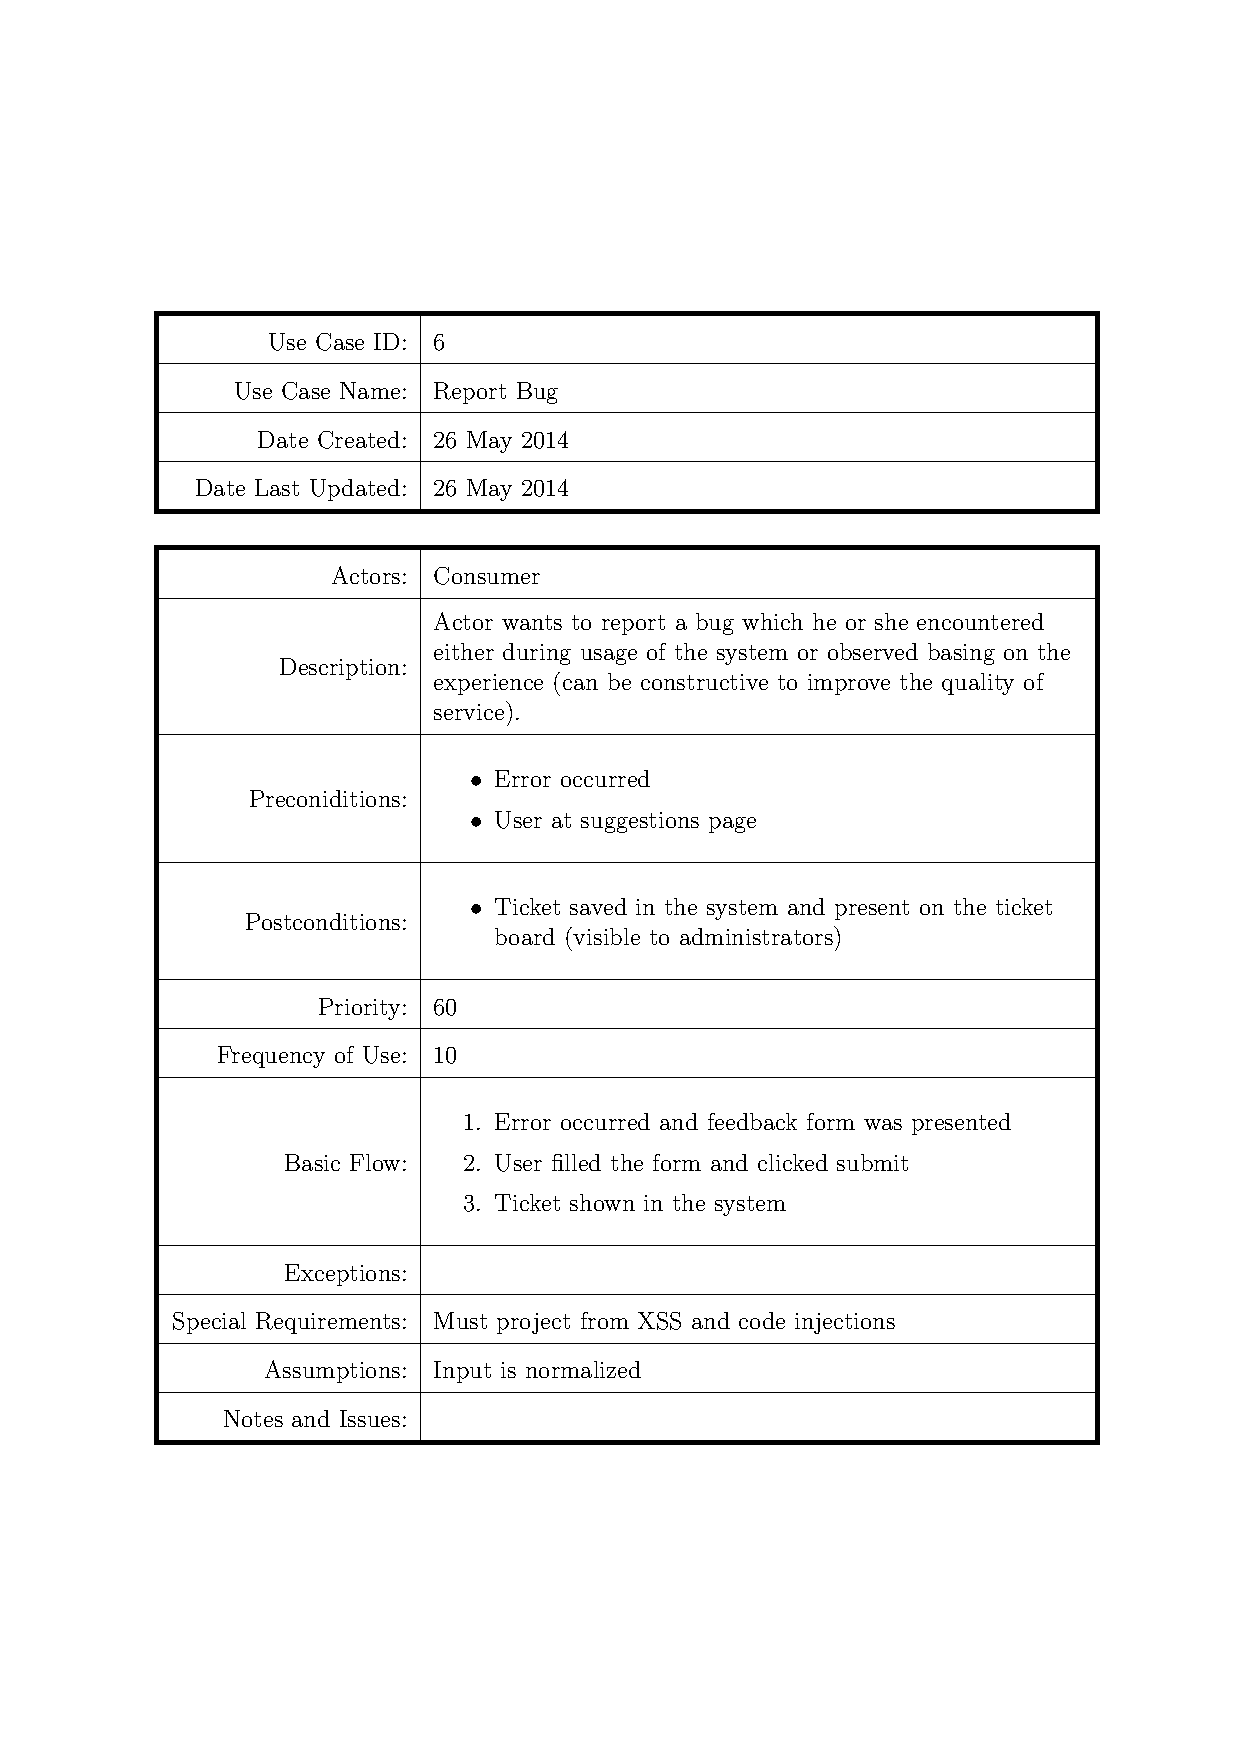
\includegraphics[width=\linewidth]{Requirements/UseCases/006_ReportBug.pdf}\end{figure*}

%---

%--- Ch3: Requirement analysis
\chapter{Requirements analysis}

\section{Objectives}
Based on the gathered requirements the following objectives were identified.
\begin{itemize}
  \item Extendibility - the project should be implemented and handled in a way that potential development into a full system should be relatively easy, i.e.
    \begin{itemize}
      \item It should be \emph{documented} (this file) and the source code should be commented that the project modules and structure should be easy to understand by a developer unfamiliar with the project;
      \item Popular technologies should be used that the potential group of developers would not be too much limit factor;
    \end{itemize}
  \item Schemaless - documents (sometimes even from the same source) will have different structure, so it is important to not restrict the database to store one kind (structure) of information, thus relational database seem as unfit solution and one of NoSQL approaches should be adopted;
  \item Open source - all technologies and tools used should be open source and the project itself should be published as open source that anyone interested should be able to use it.
\end{itemize}

\section{Structure}
Based on the objectives and requirements it was concluded that the project should be split up into the following components:
\begin{itemize}
  \item Front-End: client side code for forming queries and presenting results.
  \item Back-end: receiving queries, query processing, storing searchable data in the database and document copies.
  \item Extractor: compiling documents from different formats (e.g. PDF, DOC, TXT) without any annotations into JSON format with meta-data like contextual information from the website (e.g. document cycle, country producing, language) and structured document data, i.e. create index of sections, analyse context and information in sections and paragraph in order to create index etc.
  \item Web crawler: collecting documents for the extractor. Can be implemented as simple downloader of all files with given extension from a list of websites or general web crawler with proper seed for the documents of interest (e.g. start at MinLang committee website and Gaelic plans and follow up to 3 links).
\end{itemize}

% Fig: structure
\begin{figure*}[h]
  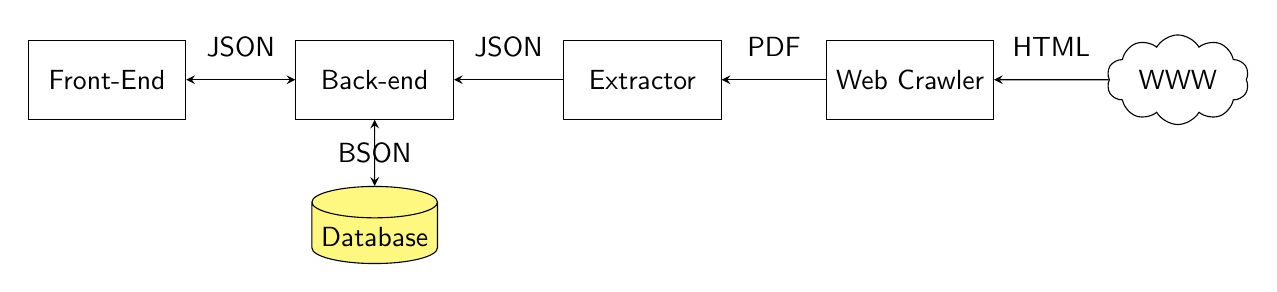
\begin{tikzpicture}[
	  decoration={
		  markings,
		  mark=at position 1cm with {\arrow[black]{stealth}},
	  },
	  path/.style={
		  ->,
		  >=stealth,
		  postaction=decorate
	  },
	  every node/.style={font=\sffamily},	
	  >=stealth,
      node distance=3.4cm,
      database/.style={
        cylinder,
        cylinder uses custom fill,
        cylinder body fill=yellow!50,
        cylinder end fill=yellow!50,
        shape border rotate=90,
        aspect=0.25,
        draw
      }
  ]

  % Boxes
  \node [
	  draw,
	  minimum width=2cm,
	  minimum height=1cm,
  ] (front) {Front-End};
  \node [
	  draw,
	  right of=front,
	  minimum width=2cm,
	  minimum height=1cm,
  ] (back) {Back-end};
  \node [
	  draw,
    right of=back,
	  minimum width=2cm,
	  minimum height=1cm,
  ] (extractor) {Extractor};
  \node [
	  draw,
    right of=extractor,
	  minimum width=2cm,
	  minimum height=1cm,
  ] (crawler) {Web Crawler};
  \node [
    cloud,
    draw,
    right of=crawler,
    cloud puffs=10,
    cloud puff arc=120,
    aspect=2
  ] (web) {WWW};

  \node[database,below of=back, node distance=2cm] (db) {Database};

  % Connecting Arrows
  \draw[<->] (front.east) -- (back.west) node [draw=none,midway,above=.5em] {JSON};
  \draw[<-] (back.east) -- (extractor.west) node [draw=none,midway,above=.5em] {JSON};
  \draw[<-] (extractor.east) -- (crawler.west) node [draw=none,midway,above=.5em] {PDF};
  \draw[<->] (db.north) -- (back.south) node [draw=none,midway] {BSON};
  \draw[<-] (crawler.east) -- (web.west) node [draw=none,midway,above=.5em] {HTML};

  \end{tikzpicture}
  
  \caption{System components}
  \label{fig:maincomps}
\end{figure*}

\section{Data layer}
\subsection{Example query}
\begin{enumerate}
  \item Show all Committee of Experts recommendations under article 7b.
  \item Show all sections relating to Scottish Gaelic.
\end{enumerate}

\subsection{Options}
The following database technologies were taken into consideration:
\begin{itemize}
  \item Traditional RDMS such as PostreSQL and MySQL
  \item Key-value store such as Riak and Redis
  \item Document database such as MongoDB and CouchDB
  \item Graph database such as Neo4J and Infinite Graph
\end{itemize}

\paragraph{Traditional RDMS} has drawback of dedicated to the outlined schema and every new document (not to mention every new source of documents) has a chance to have different organization than the previous ones.

\paragraph{Key-value store} has not enough good query languages and 

\paragraph{Document database} has both flexible structure of aggregates (so we are not dedicated to one schema) and powerful query language (which can be implemented using incremental update)

\paragraph{Graph database} has ability to perform rich queries regarding relationships, but is not as powerful when it comes to queries relating the content, can answer queries like 1 and 2 in O(1) time, but update is expensive.

\subsection{Choice}
MongoDB has been chosen for storing documents because
\begin{itemize}
  \item it has big community of supporters and developers;
  \item it is well-documented;
  \item naturally blends with JavaScript when implementing query (JQuery notation) and data from the database (JSON);
  \item can store and operate on big documents of varying schema easily
  \item has rich query language with greater capabilities than the need outlined in the example queries subsection;
  \item when used with Node.js increases programmers productivity significantly (one language, centralized view)
\end{itemize}

When developing session and account management functionality it would be beneficial to implement the concept of polyglot persistence and for these two use key-value database, which creates separation of the concers as well as suits better the case.


\section{Application layer}
\subsection{Example usage}

\subsection{Options}
Three programming languages/frameworks were considered as potentially suitable for the project, namely:
\begin{itemize}
  \item Java and JSP
  \item Python and Django
  \item JavaScript and Node.js
\end{itemize}

\paragraph{Java and JSP} does not support well the programmer productivity as to perform even the simplies operations it is very expressive. When used the application needs to be developed and tested as a whole, so it does not support modularity and extendability well. The data layer technology of choice provides API for the language, but it is rather easier and more natural to operate on it in JavaScript than in Java.

\paragraph{Python and Django} had the same drawbacks, except it provides greater productivity.

\paragraph{JavaScript and Node.js} means that one language would be used for front-end and back-end, including data quering and manipulation, what highly increases the programmer productivity. Further, JavaScript as front-end language provides rich choice of libraries like jQuery, Angular, etc. that can be used to further increase productivity and presentation quality. When it comes to the back-end all operations are handled efficiently using event-loop. The aggregates are retrieved in JSON format and MongoDB can be naturally quiered using jQuery like notation. This all results in complete and efficient solutioon.

\subsection{Choice}

Node.js has been chosen for the front-end and back-end development because
\begin{itemize}
  \item it integrates well with MongoDB
  \item enables using one language for everything (front-end, back-end, database);
  \item is efficient 
\end{itemize}

%---

%--- Ch4: Architecture
\chapter{Architecture}

\section{Overview}

\subsection{Application}

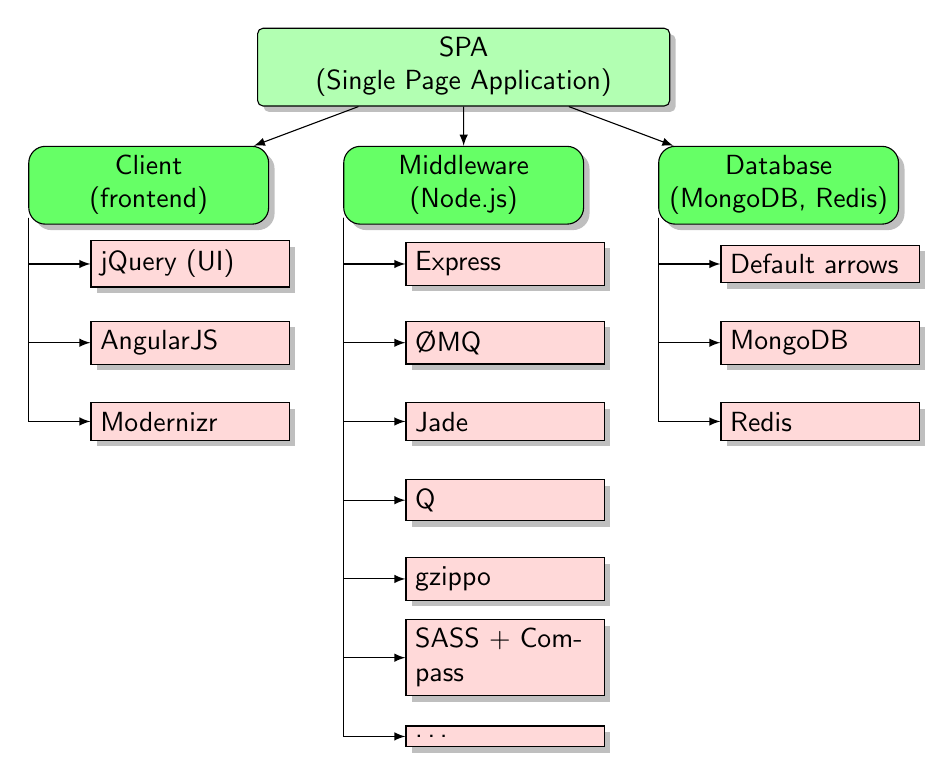
\begin{tikzpicture}[
  level 1/.style={sibling distance=40mm},
  edge from parent/.style={->,draw},
  >=latex]

% root of the the initial tree, level 1
\node[root] {SPA\\\mbox{(Single~Page~Application)}}
% The first level, as children of the initial tree
  child {node[level 2] (c1) {Client\\(frontend)}}
  child {node[level 2] (c2) {Middleware (Node.js)}}
  child {node[level 2] (c3) {Database \mbox{(MongoDB,~Redis)}}};

% The second level, relatively positioned nodes
\begin{scope}[every node/.style={level 3}]
\node [below of = c1, xshift=15pt] (c11) {jQuery (UI)};
\node [below of = c11] (c12) {AngularJS};
\node [below of = c12] (c13) {Modernizr};

\node [below of = c2, xshift=15pt] (c21) {Express};
\node [below of = c21] (c22) {{\O}MQ};
\node [below of = c22] (c23) {Jade};
\node [below of = c23] (c24) {Q};
\node [below of = c24] (c25) {gzippo};
\node [below of = c25] (c26) {SASS + Compass};
\node [below of = c26] (c27) {\dots};

\node [below of = c3, xshift=15pt] (c31) {Default arrows};
\node [below of = c31] (c32) {MongoDB};
\node [below of = c32] (c33) {Redis};
\end{scope}

% lines from each level 1 node to every one of its "children"
\foreach \value in {1,2,3}
  \draw[->] (c1.195) |- (c1\value.west);

\foreach \value in {1,...,7}
  \draw[->] (c2.195) |- (c2\value.west);

\foreach \value in {1,...,3}
  \draw[->] (c3.195) |- (c3\value.west);
\end{tikzpicture}

Description
\begin{itemize}
\item [\textbf{Client:}]
  \item jQuery (UI)
  \item AngularJS
  \item Modernizr

\item [\textbf{Middleware:}]  
  \item Express - main framework for message passing and service the content to the clients
  \item {\O}MQ - for message passing, mainly for efficient Router/Dealer protocol implementation
  \item Jade - for more productivity in templating
  \item gzippo - for serving gzipped content
  \item SASS + Compass - styling, plus features like building sprites out of files

\item [\textbf{Database:}]
  \item MongoDB - document data store for document management \emph{TODO}
  \item Redis - key-value data store for session and user data management
\end{itemize}

\subsection{Full layer}
% TODO: Add packages description and links to the project websites, and icons :)
\emph{Picture showing Yeoman, Grunt, Karma testing with Jasmin, etc.}
code: sudo npm install -g yo \# installs yeoman, grunt, bower, etc. globally
sudo npm install -g generator-angular-fullstack \# install angular generator (btw the most popular generator)
yo angular-fullstack seeker (projectname)\# create full stack locally with jade tempalates
[?] Would you like to use Sass (with Compass)? Yes                               │
[?] Would you like to include Twitter Bootstrap? Yes                             │
[?] Would you like to use the Sass version of Twitter Bootstrap? Yes             │
[?] Which modules would you like to include?                                     │
‣⬢ angular-resource.js                                                           │
 ⬢ angular-cookies.js                                                            │
 ⬢ angular-sanitize.js                                                           │
 ⬢ angular-route.js 
 mongo with mongosee
 passport 
 All yeses
\subsection{Code management and deployment process}

\section{Full stack}
\subsection{Client facing}
\subsection{Middleware}
\subsection{Persistence data store}


\section{System design}

\section{Query language}

\subsection{Elements}
\begin{itemize}
  \item \emph{source documents} (e.g. Committee of Experts reports)
  \item \emph{document specifiers} (e.g. cycle, country producing the document)
  \item \emph{selectors} (i.e., languages, sections, words)
  \item \emph{organizer} specifying how to structure the output document (e.g. arrange by section numbers, in each section by countries alphabetically)
  \item \emph{template} choose how to style the output document
\end{itemize}

\subsection{Dependencies as tree}
\begin{enumerate}
  \item \emph{Source documents} must be root.
  \item \emph{Document specifiers} can be children of each another, but can occur only once on any path from root to leaves, can appear multiple times.
  \item \emph{Selectors} (i.e. languages, sections, words) can be children of any node, and they are always terminal (leaves).
  \item \emph{Organizers}, \emph{templates}, and other similar options which can be added in the future must be children of root, and in case of \emph{organizers} they must be aware of all root's children except itself to display available options.
\end{enumerate}

\subsection{Query evaluation stages}
\begin{enumerate}
  \item Select relevant documents using:
  \begin{itemize}
    \item producer - group (e.g. committee)
    \item producer - origin, i.e. countries (e.g. UK)
    \item cycles - time (e.g. last)
  \end{itemize}
  \item filter the document content using selectors (i.e. sections, languages, filters- words, phrases, etc.)
  \item reorganize resulting JSON using organizers
  \item render using template
\end{enumerate}


%---
% Ch5: Implementation

\section{Implementation}
\subsection{Core}
% node.js + zmq + angularjs + mongodb ^ mongoose
\subsection{Rendering}
% compass + Sass
\subsection{Auxiliary modules}

%---
% Ch6: Deployment

\section{Deployment}
\subsection{Hosting Environment}
% vm on plaistow
% config
\subsection{Connecting to the server}
% ssh into user -> telnet into seeker/plaistow (machine)
\subsection{Managing Modules}
% localization due to restricted privileges
\subsection{Deployment Cycle}
% test -> sync -> restart
\subsection{Testing}
% test server
\subsection{Persistence}
% auto reboot with grunt.js

%---
% Ch7: Available data

\section{Data}

%---
% Ch8: Project perspectives

\section{Perspectives}

\end{document}